% !TeX program = pdfLaTeX
\documentclass[12pt]{article}
\usepackage{amsmath}
\usepackage{graphicx,psfrag,epsf}
\usepackage{enumerate}
\usepackage{natbib}
\usepackage{textcomp}
\usepackage[hyphens]{url} % not crucial - just used below for the URL
\usepackage{hyperref}

%\pdfminorversion=4
% NOTE: To produce blinded version, replace "0" with "1" below.
\newcommand{\blind}{0}

% DON'T change margins - should be 1 inch all around.
\addtolength{\oddsidemargin}{-.5in}%
\addtolength{\evensidemargin}{-.5in}%
\addtolength{\textwidth}{1in}%
\addtolength{\textheight}{1.3in}%
\addtolength{\topmargin}{-.8in}%

%% load any required packages here



% tightlist command for lists without linebreak
\providecommand{\tightlist}{%
  \setlength{\itemsep}{0pt}\setlength{\parskip}{0pt}}



\usepackage[dvipsnames]{xcolor} % colors
\newcommand{\ear}[1]{{\textcolor{blue}{#1}}}
\newcommand{\svp}[1]{{\textcolor{RedOrange}{#1}}}
\newcommand{\rh}[1]{{\textcolor{Green}{#1}}}
\usepackage[capitalise]{cleveref}
\newcommand\pcref[1]{(\cref{#1})}
\usepackage{algorithm,algpseudocode,booktabs}

\begin{document}


\def\spacingset#1{\renewcommand{\baselinestretch}%
{#1}\small\normalsize} \spacingset{1}


%%%%%%%%%%%%%%%%%%%%%%%%%%%%%%%%%%%%%%%%%%%%%%%%%%%%%%%%%%%%%%%%%%%%%%%%%%%%%%

\if0\blind
{
  \title{\bf Perception of Curvature \& Exponential Growth}

  \author{
        Emily A. Robinson 1 \\
    Department of Statistics, California Polytechnic State University -
San Luis Obispo\\
     and \\     Reka Howard 2 \\
    Department of Statistics, University of Nebraska - Lincoln\\
     and \\     Susan VanderPlas 3 \\
    Department of Statistics, University of Nebraska - Lincoln\\
      }
  \maketitle
} \fi

\if1\blind
{
  \bigskip
  \bigskip
  \bigskip
  \begin{center}
    {\LARGE\bf Perception of Curvature \& Exponential Growth}
  \end{center}
  \medskip
} \fi

\bigskip
\begin{abstract}
The text of your abstract. 200 or fewer words.
\end{abstract}

\noindent%
{\it Keywords:} log scales, visual inference, graphical testing
\vfill

\newpage
\spacingset{1.45} % DON'T change the spacing!

\hypertarget{introduction}{%
\section{Introduction}\label{introduction}}

Effective communication of data is critical in influencing people's
opinions and actions. This was particularly true during the COVID-19
pandemic, where data visualizations and dashboards played a vital role
in informing the public and policymakers about the status of the
outbreak. Local governments relied on graphics to inform their decisions
about shut downs and mask mandates, while residents were presented with
data visualizations to encourage compliance with these regulations. A
major issue we encountered in the creation of COVID-19 plots was how to
display data from a wide range of values. When faced with data which
spans several orders of magnitude, we must decide whether to show the
data on its original scale (compressing the smaller magnitudes into
relatively little area) or to transform the scale and alter the
contextual appearance of the data. Log scale transformations have
emerged as a common solution to this challenge, as they allow for the
display of data over several orders of magnitude within a single graph.

Exponential curves are a common source of data in which smaller
magnitudes are compressed into a smaller area, as illustrated by Fig.
1.16, which presents an exponential curve displayed on both linear and
log scales to demonstrate the usefulness of log scales when dealing with
data that spans multiple magnitudes. Logarithms facilitate the
conversion of multiplicative relationships (such as 1 \& 10 being
displayed 10 units apart and 10 \& 100 being displayed 90 units apart)
to additive relationships (such as 1 \& 10, and 10 \& 100, being evenly
spaced along the axis), highlighting proportional relationships and
linearizing power functions \citep{menge_logarithmic_2018}. Logarithms
also have practical applications, simplifying the computation of small
numbers like likelihoods and transforming data to conform to statistical
assumptions. Although log scales have a long history of use in fields
such as ecology, psychophysics, engineering, and physics
\citep{heckler_student_2013, waddell2005comparisons}, there is still a
need to understand the implications of their use and provide best
practices for their implementation.

In this paper, we evaluate the benefits and drawbacks of using log
scales and examine their impact on perceptual sensitivity by conducting
a visual inference experiment using statistical lineups
\citep{buja_statistical_2009}. The experiment focused on a participants
ability to identify differences between exponentially increasing curves
with varying levels of curvature, using both linear and log scales.
Participants did not require any mathematical training or understanding
of exponential growth or logarithmic scales to participate in the study,
highlighting the fundamental nature of the ability to identify
differences in charts. This study lays the groundwork for further
exploration of the implications of using log scales in data
visualization.

\hypertarget{statistical-lineups}{%
\subsection{Statistical Lineups}\label{statistical-lineups}}

A data plot can be evaluated and treated as a visual statistic, a
numerical function which summarizes the data. To evaluate a graph, the
statistic (data plot) must be run through a visual evaluation - a
person. We can conclude that two visualization methods are significantly
different if the visual evaluation is different. Recent graphical
experiments have utilized statistical lineups to quantify the perception
of graphical design choices
\citep{hofmann_graphical_2012, loy_model_2017, loy_variations_2016, vanderplas_clusters_2017}.
Statistical lineups provide an elegant way of combining perception and
statistical hypothesis testing using graphical experiments
\citep{majumder_validation_2013, vanderplas_testing_2020, wickham2010graphical}.
`Lineups' are named after the `police lineup' of criminal investigations
where witnesses are asked to identify the criminal from a set of
individuals. Similarly, a statistical lineup is a plot consisting of
smaller panels where the viewer is asked to identify the panel
containing the real data from among a set of decoy null plots. Null
plots display data under the assumption there is no relationship and can
be generated by permutation or simulation. A statistical lineup
typically consists of 20 panels - one target panel and 19 null panels.
If the viewer can identify the target panel randomly embedded within the
set of null panels, this suggests that the real data is visually
distinct from data generated under the null model.
\cref{fig:lineup-example} provides examples of statistical lineups. The
lineup plot on the left displays increasing exponential data displayed
on a linear scale with panel 13 as the target; the lineup plot on the
right displays increasing exponential data on the log base ten scale
with panel 4 as the target.

\begin{verbatim}
## Warning: The `size` argument of `element_rect()` is deprecated as of
## ggplot2 3.4.0.
## i Please use the `linewidth` argument instead.
\end{verbatim}

\begin{figure}[tbp]

{\centering 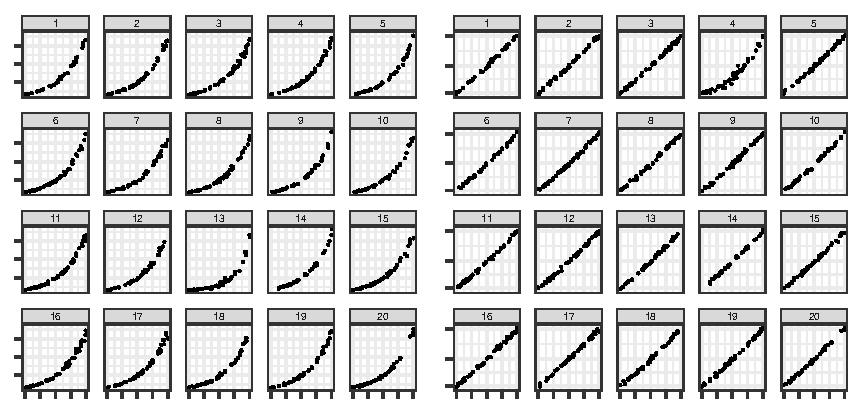
\includegraphics[width=\linewidth,]{logarithmic-lineups_files/figure-latex/lineup-example-1} 

}

\caption[Lineup examples]{The lineup plot on the left displays increasing exponential data on a linear scale with panel (2 x 5) + 3 as the target. The lineup plot on the right displays increasing exponential data on the log scale with panel 2 x 2 as the target.}\label{fig:lineup-example}
\end{figure}

While explicit graphical tests direct the participant to a specific
feature of a plot to answer a specific question, implicit graphical
tests require the user to identify both the purpose and function of the
plot in order to evaluate the plots shown
\citep{vanderplas_testing_2020}. Implicit graphical tests, such as
lineups, have the advantage of simultaneously visually testing for
multiple visual features including outliers, clusters, linear and
nonlinear relationships. Responses from multiple viewers are collected
through convenience sampling (in informal situations) or crowd sourcing
websites such as Prolific, Amazon Mechanical Turk, and Reddit (in more
formal situations).

\hypertarget{study-development}{%
\section{Study Development}\label{study-development}}

\hypertarget{data-generation}{%
\subsection{Data Generation}\label{data-generation}}

In this study, both the target and null data sets were generated by
simulating data from an exponential model; the models differ in the
parameters selected for the null and target panels. In order to
guarantee the simulated data spans the same domain and range of values,
we began with a domain constraint of \(x\in [0,20]\) and a range
constraint of \(y\in [10,100]\) with \(N = 50\) points randomly assigned
throughout the domain and mapped to the \(y\)-axis using the exponential
model with the selected parameters. These constraints provide some
assurance that participants who select the target plot are doing so
because of their visual perception differentiating between curvature or
growth rate rather than different starting or ending values.

Data were simulated based on a three-parameter exponential model with
multiplicative errors: \begin{align}
y_i & = \alpha\cdot e^{\beta\cdot x_i + \epsilon_i} + \theta \\
\text{with } \epsilon_i & \sim N(0, \sigma^2). \nonumber
\end{align} The parameters \(\alpha\) and \(\theta\) were adjusted based
on \(\beta\) and \(\sigma^2\) to guarantee the range and domain
constraints are met. The model generated \(N = 50\) points
\((x_i, y_i), i = 1,...,N\) where \(x\) and \(y\) have an increasing
exponential relationship. The heuristic data generation procedure is
described in \cref{alg:lineup-parameter-estimation-algorithm} and
\cref{alg:lineup-exponential-data-simulation-algorithm}.

\begin{algorithm}
  \caption{Lineup Parameter Estimation}\label{alg:lineup-parameter-estimation-algorithm}
  \begin{algorithmic}[1]
    \Statex \textbullet~\textbf{Input Parameters:} domain $x\in[0,20]$, range $y\in[10,100]$, midpoint $x_{mid}$.
    \Statex \textbullet~\textbf{Output Parameters:} estimated model parameters $\hat\alpha, \hat\beta, \hat\theta$.
    \State Determine the $y=-x$ line scaled to fit the assigned domain and range.
    \State Map the values $x_{mid} - 0.1$ and $x_{mid} + 0.1$ to the $y=-x$ line for two additional points.
    \State From the set of points $(x_k, y_k)$ for $k = 1,2,3,4$, calculate the coefficients from the linear regression model $\ln(y_k) = b_0 +b_1x_k$ to obtain starting values - $\alpha_0 = e^{b_0}, \beta_0 =  b_1, \theta_0 = 0.5\cdot \min(y)$
    \State Using the \texttt{nls} function from the base \texttt{stats} package in Rstudio and the starting parameter values - $\alpha_0, \beta_0, \theta_0$ - fit the nonlinear model, $y_k = \alpha\cdot e^{\beta\cdot x_k}+\theta$ to get estimated parameter values - $\hat\alpha, \hat\beta, \hat\theta.$
  \end{algorithmic}
\end{algorithm}

\begin{algorithm}
  \caption{Lineup Exponential Data Simulation}\label{alg:lineup-exponential-data-simulation-algorithm}
  \begin{algorithmic}[1]
    \Statex \textbullet~\textbf{Input Parameters:} sample size $N = 50$, estimated parameters $\hat\alpha$, $\hat\beta$, and $\hat\theta$, from \cref{alg:lineup-parameter-estimation-algorithm}, and standard deviation $\sigma$ from the exponential curve.
    \Statex \textbullet~\textbf{Output Parameters:} $N$ points, in the form of vectors $\mathbf{x}$ and $\mathbf{y}$.
    \State Generate $\tilde x_j, j = 1,..., \frac{3}{4}N$ as a sequence of evenly spaced points in $[0,20]$. This ensures the full domain of $x$ is used, fulfilling the constraints of spanning the same domain and range for each parameter combination.
    \State Obtain $\tilde x_i, i = 1,...N$ by sampling $N = 50$ values from the set of $\tilde x_j$ values. This guarantees some variability and potential clustering in the exponential growth curve disrupting the perception due to continuity of points.
    \State Obtain the final $x_i$ values by jittering $\tilde x_i$.
    \State Calculate $\tilde\alpha = \frac{\hat\alpha}{e^{\sigma^2/2}}.$ This ensures that the range of simulated values for different standard deviation parameters has an equal expected value for a given rate of change due to the non-constant variance across the domain.
    \State Generate $y_i = \tilde\alpha\cdot e^{\hat\beta x_i + e_i}+\hat\theta$ where $e_i\sim N(0,\sigma^2).$
  \end{algorithmic}
\end{algorithm}

\hypertarget{lineups-parameter-selection}{%
\subsection{Parameter Selection}\label{lineups-parameter-selection}}

We followed a `Goldilocks' inspired procedure to choose three levels of
trend curvature (low curvature, medium curvature, and high curvature).
For each curvature level, we simulated 1,000 data sets of
\((x_{ij}, y_{ij})\) points for \(i = 1,...,50\) increments of
\(x\)-values and replicate \(j = 1,...,10\) corresponding \(y\)-values
per \(x\)-value. Each generated \(x_i\) point from
\cref{alg:lineup-exponential-data-simulation-algorithm} was replicated
ten times. On each of the individual data sets, we fit a linear
regression model and computed the lack of fit statistic (LOF) which
measures the deviation of the data from the linear regression model. The
density curves of the LOF statistics for each level of curvature are
plotted (\cref{fig:lof-density-curves}) to provide a metric for
differentiating between the curvature levels and thus detecting the
target plot. While the LOF statistic provides a numerical value for
discriminating between the difficulty levels, it cannot be directly
related to the perceptual discriminability; it serves primarily as an
approximation to ensure that we are testing parameters at several
distinct curvature levels. Final parameters used for data simulation are
shown in \cref{tab:parameter-data}.

\begin{figure}[tbp]

{\centering 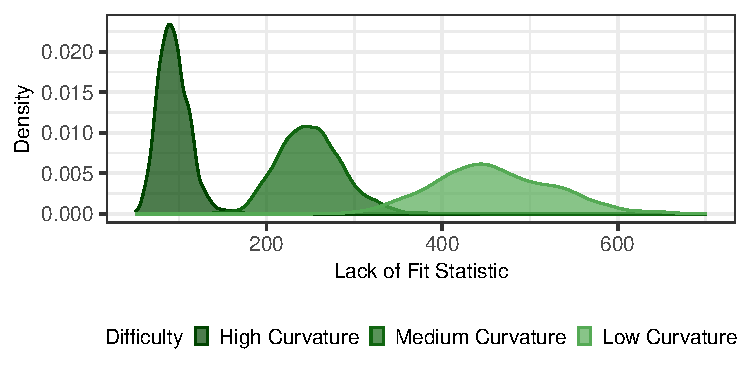
\includegraphics[width=1\linewidth,]{logarithmic-lineups_files/figure-latex/lof-density-curves-1} 

}

\caption[Lineup parameter selection]{Density plot of the lack of fit statistic showing separation of difficulty levels: obvious curvature, noticable curvature, and almost linear.}\label{fig:lof-density-curves}
\end{figure}

\begin{table}

\caption{\label{tab:parameter-data}Lineup data simulation final parameters}
\centering
\begin{tabular}[t]{ccccccc}
\toprule
 & $x_{mid}$ & $\hat\alpha$ & $\tilde\alpha$ & $\hat\beta$ & $\hat\theta$ & $\hat\sigma$\\
\midrule
High Curvature & 14.5 & 0.91 & 0.88 & 0.23 & 9.10 & 0.25\\
Medium Curvature & 13.0 & 6.86 & 6.82 & 0.13 & 3.14 & 0.12\\
Low Curvature & 11.5 & 37.26 & 37.22 & 0.06 & -27.26 & 0.05\\
\bottomrule
\end{tabular}
\end{table}

\hypertarget{lineup-setup}{%
\subsection{Lineup Setup}\label{lineup-setup}}

Lineup plots were generated by mapping one simulated data set
corresponding to curvature level A to a scatter plot to be identified as
the target panel while multiple simulated data sets corresponding to
curvature level B were individually mapped to scatter plots for the null
panels. The \texttt{nullabor} package in R \citep{nullabor} was used to
randomly assign the target plot to one of the panels surrounded by
panels containing null plots. For example, a target plot with simulated
data following an increasing exponential curve with high curvature is
randomly embedded within null plots with simulated data following an
increasing exponential trend with low curvature. By the implemented
constraints, the target panel and null panels spanned a similar domain
and range. There were a total of six lineup curvature combinations;
\cref{fig:curvature-combination-example} illustrates the six lineup
curvature combinations (top: linear scale; bottom: log scale) where the
green line indicates the curvature level designated to the target plot
while the black line indicates the curvature level assigned to the null
plots. Two sets of each lineup curvature combination were simulated
(total of twelve test data sets) and plotted on both the linear scale
and the log scale (total of 24 test lineup plots). In addition, there
were three curvature combinations which generated homogeneous
``Rorschach'' lineups, where all panels were from the same distribution.
Each participant evaluated one of these lineups, but for simplicity,
these evaluations are not described in this chapter and their analysis
is left to a later date.

\begin{verbatim}
## Warning: Using `size` aesthetic for lines was deprecated in ggplot2
## 3.4.0.
## i Please use `linewidth` instead.
\end{verbatim}

\begin{figure}[tbp]

{\centering 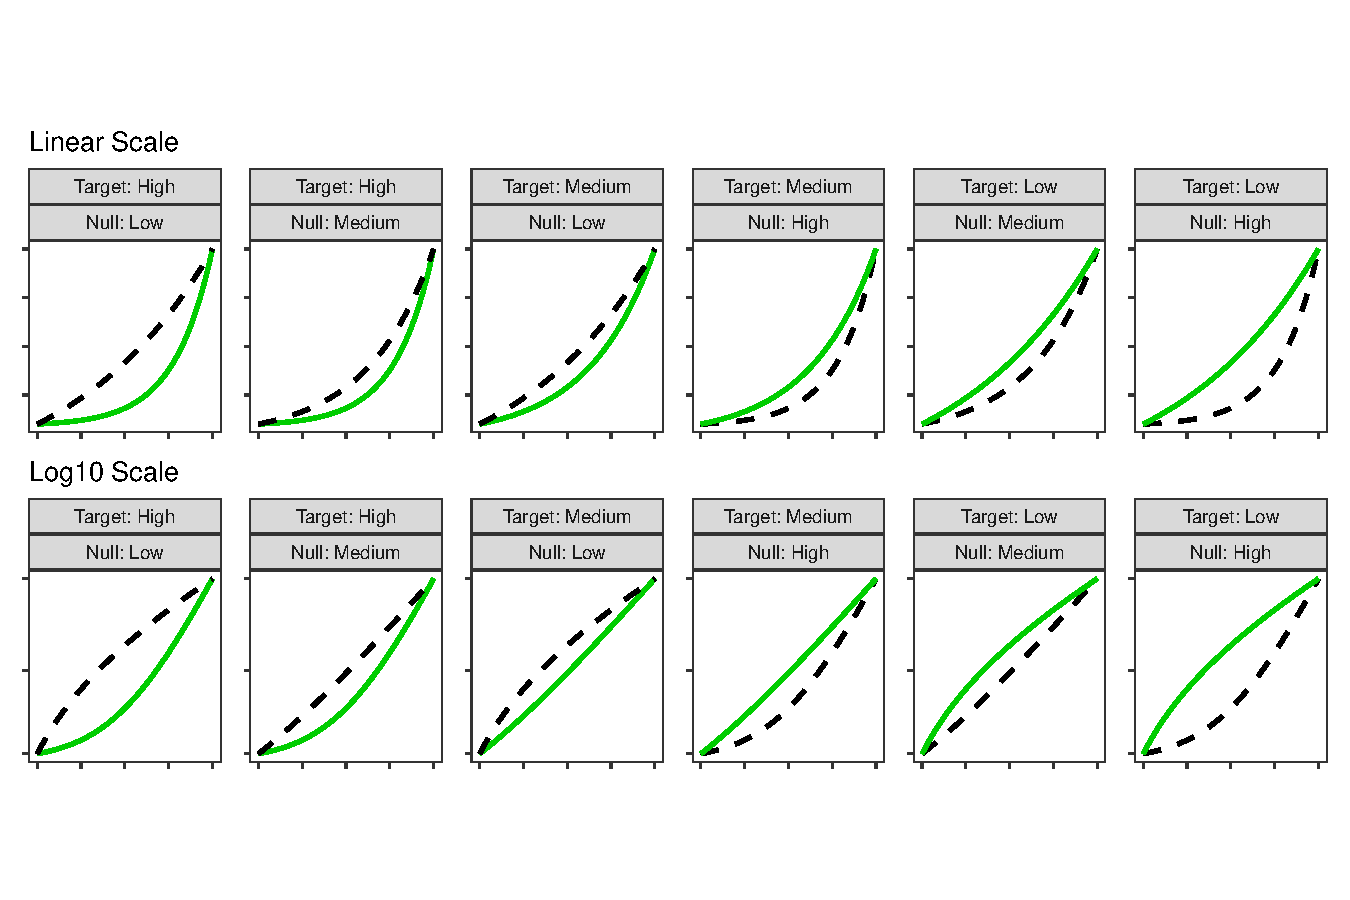
\includegraphics[width=1\linewidth,]{logarithmic-lineups_files/figure-latex/curvature-combination-example-1} 

}

\caption[Lineup curvature combinations]{Thumbnail plots illustrating the six curvature combinations displayed on both scales (linear and log). The green line indicates the curvature level to be identified as the target plot from amongst a set of null plots with the curvature level indicated by the black line.}\label{fig:curvature-combination-example}
\end{figure}

\hypertarget{study-design}{%
\subsection{Study Design}\label{study-design}}

Each participant was shown a total of thirteen lineup plots (twelve test
lineup plots and one Rorschach lineup plot). Participants were randomly
assigned one of the two replicate data sets for each of the six unique
lineup curvature combinations. For each assigned test data set, the
participant was shown the lineup plot corresponding to both the linear
scale and the log scale. For the additional Rorschach lineup plot,
participants were randomly assigned one data set shown on either the
linear or the log scale. The order of the thirteen lineup plots shown
was randomized for each participant.

Participants above the age of majority in their region were recruited
from Prolific, a survey site that connects researchers to study
participants. Participants were compensated for their time and
participated in all three related graphical studies consecutively.
Previous literature suggests that prior mathematical knowledge or
experience with exponential data is not associated with the outcome of
graphical experiments involving lineups\citep{vanderplas2015spatial}.
The lineup study in this chapter was completed first in the series of
graphical studies.

Participants were shown a series of lineup plots and asked to identify
the plot that was most different from the others. On each plot,
participants were asked to justify their choice and provide their level
of confidence in their choice. The goal of this graphical task was to
test an individual's ability to perceptually differentiate exponentially
increasing trends with differing levels of curvature on both the linear
and log scale.

\hypertarget{results}{%
\section{Results}\label{results}}

Participant recruitment and study deployment were conducted via
Prolific, a crowd sourcing website, on Wednesday, March 23, 2022 during
which 325 individuals completed 4,492 unique test lineup evaluations.
Only participants who completed the lineup study were included in the
final data set which included a total of 311 participants and 3,958
lineup evaluations. Each plot was evaluated between 141 and 203 times
(Mean: 164.92, SD: 14.9). Participants correctly identified the target
panel in 47\% of the 1,981 lineup evaluations made on the linear scale
and 65.3\% of the 1,977 lineup evaluations made on the log scale.

Each lineup plot evaluated was assigned a binary value based on the
participant response (correct target plot identification = 1, not
correct target plot identification = 0). We defined \(Y_{ijkl}\) to be
the event that participant \(l = 1,...,N_\text{participant}\) correctly
identified the target plot for data set \(k = 1,2\) with curvature
combination \(j = 1,2,3,4,5,6\) plotted on scale \(i = 1,2\). The binary
response was analyzed using a generalized linear mixed model (GLMM)
following a binomial distribution with a logit link function with a
row-column blocking design accounting for the variation due to
participant and data set respectively as \begin{equation}
\text{logit }P(Y_{ijk}) = \eta + \delta_i + \gamma_j + \delta \gamma_{ij} + s_l + d_k
\end{equation} \noindent where

\begin{itemize}
\item $\eta$ is the baseline average probability of selecting the target plot
\item $\delta_i$ is the effect of scale $i = 1,2$
\item $\gamma_j$ is the effect of curvature combination $j = 1,2,3,4,5,6$
\item $\delta\gamma_{ij}$ is the two-way interaction between the $i^{th}$ scale and $j^{th}$ curvature combination
\item $s_l \sim N(0,\sigma^2_\text{participant})$ is the random effect for participant characteristics
\item $d_k \sim N(0,\sigma^2_{\text{data}})$ is the random effect for data specific characteristics. 
\end{itemize}

\noindent We assumed that random effects for data set and participant
are independent. Target plot identification was analyzed using a GLMM
implemented in \texttt{glmer} from the \texttt{lme4} R package
\citep{lme4}. Estimates and odds ratio comparisons between the log and
linear scales were calculated using the \texttt{emmeans} R package
\citep{emmeans}.

Results indicated a strong interaction between the curvature combination
and scale (\(\chi^2_5 = 294.443\); \(\text{p} <0.0001\)). Variance due
to participant and data set were estimated to be
\(\hat\sigma^2_{\text{participant}} = 1.19\) (s.e. = 1.09) and
\(\hat\sigma^2_{\text{data}} = 0.433\) (s.e. = 0.66), respectively.

On both the log and linear scales, the highest accuracy occurred in
lineup plots where the target model and null model had a large curvature
difference and the target plot had more curvature than the null plots
(high curvature target plot embedded in low curvature null plots). There
is a decrease in accuracy on the linear scale when comparing a target
plot with less curvature to null plots with more curvature (medium
curvature target plot embedded in high curvature null plots; low
curvature target plot embedded in medium curvature null plots; low
curvature target plot embedded in high curvature null plots).
\citet{best_perception_2007} found that accuracy of identifying the
correct curve type was higher when nonlinear trends were presented
indicating that it is hard to say something is linear (something has
less curvature), but easy to say that it is not linear; our results
concur with this observation. \cref{fig:odds-ratio-plot} displays the
estimated (log) odds ratio of successfully identifying the target panel
on the log scale compared to the linear scale. The thumbnail figures to
the right of the plot illustrate the curvature combination on both the
linear (left thumbnail) and log base ten (right thumbnail) scales
associated with the \(y\)-axis label. The choice of scale had no impact
if curvature differences are large and the target plot had more
curvature than the null plots (high curvature target plot embedded in
low curvature null plots). However, presenting data on the log scale
makes us more sensitive to slight changes in curvature (low or high
curvature target plot embedded in medium curvature null plots; medium
curvature target plot embedded in high curvature null plots) and large
differences in curvature when the target plot had less curvature than
the null plots (low curvature target plot embedded in high curvature
null plots). An exception occured when identifying a plot with curvature
embedded in null plots close to a linear trend (medium curvature target
panel embedded in low curvature null panels). The results indicate that
participants were more accurate at detecting the target panel on the
linear scale than the log scale. When examining this curvature
combination, the same perceptual effect occurred as what we previously
saw, but in a different context of scales. On the linear scale,
participants were perceptually identifying a curved trend from close to
a linear trend whereas after the logarithmic transformation,
participants were perceptually identifying a trend close to linear from
a curved trend. This again supports the claim that it is easy to
identify a curve in a bunch of lines but harder to identify a line in a
bunch of curves \citep{best_perception_2007}.

\begin{figure}[tbp]

{\centering 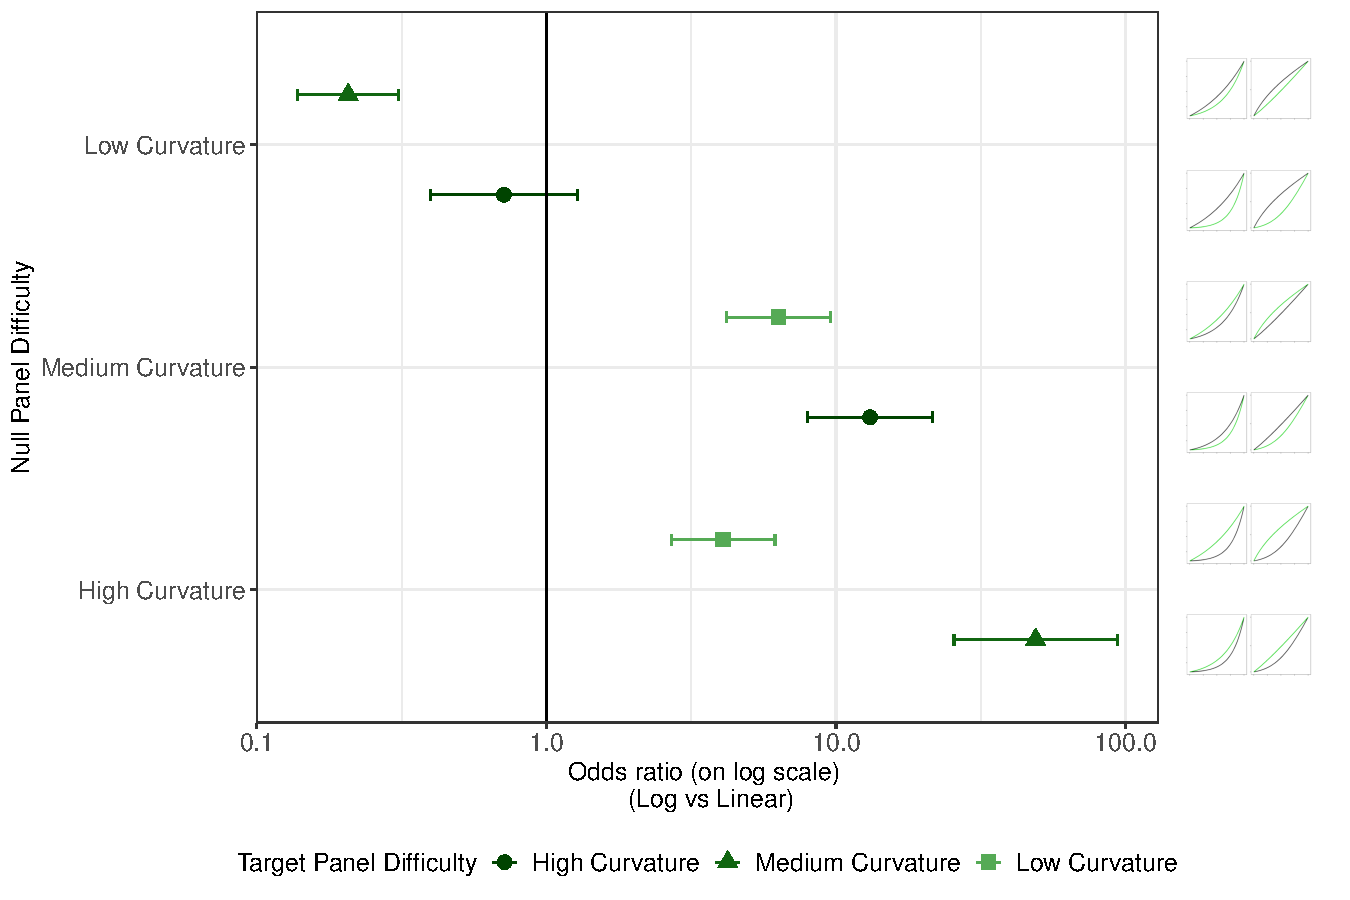
\includegraphics[width=\linewidth,]{logarithmic-lineups_files/figure-latex/odds-ratio-plot-1} 

}

\caption[Lineups log(odds) results]{Estimated (log) odds ratio of successfully identifying the target panel on the log scale compared to the linear scale. The y-axis indicates the the model parameters used to simulate the null plots with the target plot model parameter selection designated by shape and shade of green. The thumbnail figures on the right display the curvature combination as shown in \cref{fig:curvature-combination-example} on both scales (linear - left, log - right).}\label{fig:odds-ratio-plot}
\end{figure}

\hypertarget{discussion-and-conclusion}{%
\section{Discussion and Conclusion}\label{discussion-and-conclusion}}

The overall goal of this chapter is to provide basic research to support
the principles used to guide design decisions in scientific
visualizations of exponential data. In this study, we explored the use
of linear and log scales to determine whether our ability to notice
differences in exponentially increasing trends is impacted by the choice
of scale. The results indicated that when there was a large difference
in curvature between the target plot and null plots and the target plot
had more curvature than the null plots, the choice of scale had no
impact and participants accurately differentiated between the two curves
on both the linear and log scale. However, displaying exponentially
increasing data on a log scale improved the accuracy of differentiating
between models with slight curvature differences or large curvature
differences when the target plot had less curvature than the null plots.
An exception occurred when identifying a plot with curvature embedded in
surrounding plots closely relating to a linear trend, indicating that it
is easy to identify a curve in a group of lines but much harder to
identify a line in a group of curves. The use of visual inference to
identify these guidelines suggests that there are \emph{perceptual}
advantages to log scales when differences are subtle. What remains to be
seen is whether there are cognitive disadvantages to log scales: do log
scales make it harder to make use of graphical information?

\bibliographystyle{agsm}
\bibliography{bibliography.bib}


\end{document}
